\documentclass[margin=5pt]{standalone}
\usepackage{tikz}
\usetikzlibrary{calc}
\tikzset{
  my edge from parent fork down/.style={
    edge from parent path={
      (\tikzparentnode\tikzparentanchor)
      -- ($(\tikzparentnode.south)!0.5!(\tikzchildnode.north-|\tikzparentnode.south)$)
      -| (\tikzchildnode\tikzchildanchor)
    }}
  }

\begin{document}

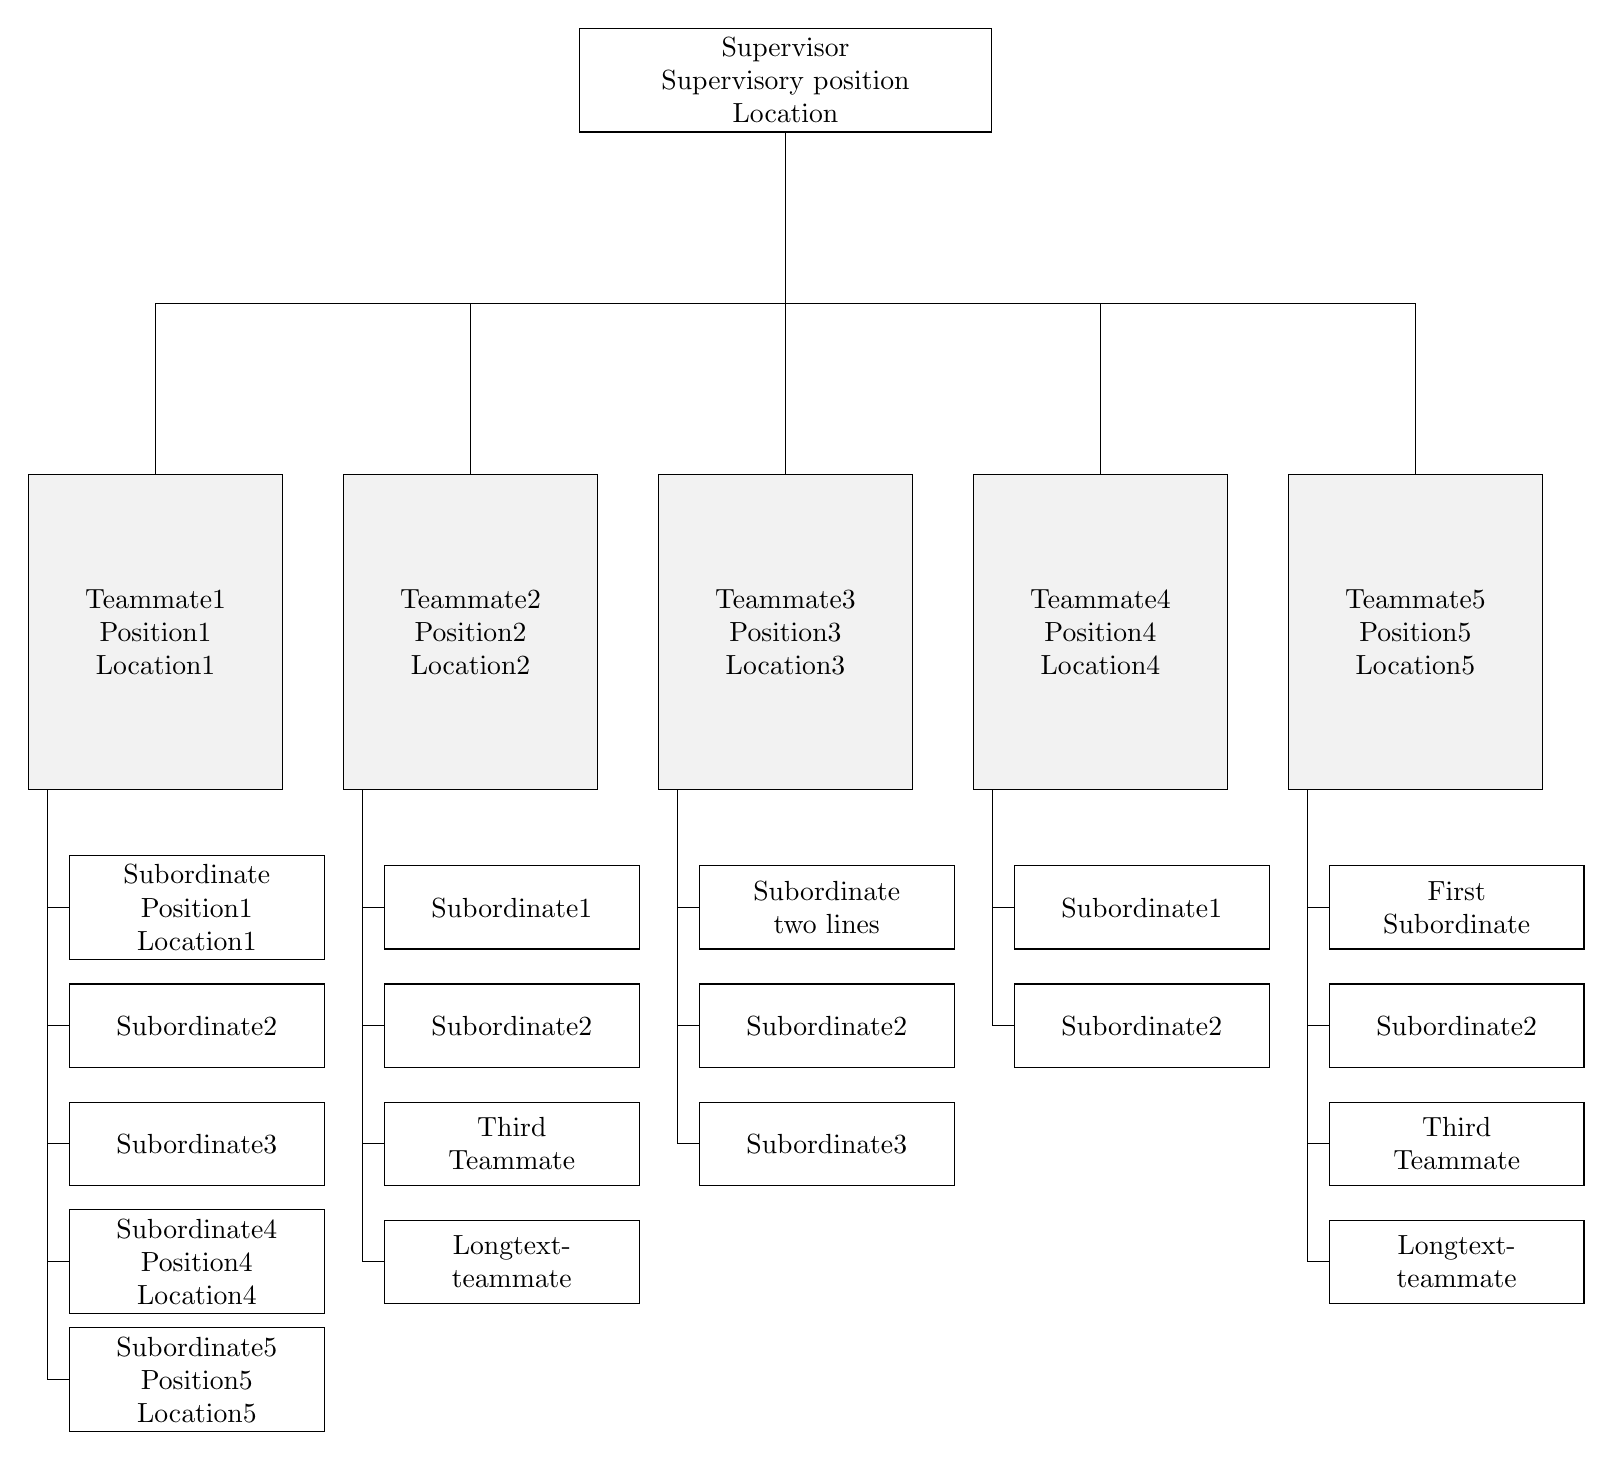
\begin{tikzpicture}[
    nodes={draw=black, thin,minimum height=3em},
    supervisor/.style={%
        text centered, text width=5cm},
    teammate/.style={%
        text centered, text width=3cm,
        minimum height=4cm,anchor=north,
        fill=gray!10},
    subordinate/.style={%
        anchor=west,
        grow=down, xshift=-1.1cm, % Horizontal position of the child node
        text centered, text width=3cm,
        edge from parent path={([xshift=-1.375cm]\tikzparentnode.south) |- (\tikzchildnode.west)}},
    level1/.style ={level distance=3.5cm},
    level2/.style ={level distance=5cm},
    level3/.style ={level distance=6.5cm},
    level4/.style ={level distance=8cm},
    level5/.style ={level distance=9.5cm},
    level 1/.style={sibling distance=4cm,level distance=5cm},
]
    % Supervisor
    \node[anchor=south,supervisor]{Supervisor\\Supervisory position\\Location}
    [my edge from parent fork down]
    % Teammate and Subordinates
    child{node [teammate] {Teammate1\\Position1\\Location1}
        child[subordinate,level1] {node {Subordinate\\Position1\\Location1}}
        child[subordinate,level2] {node {Subordinate2}}
        child[subordinate,level3] {node {Subordinate3}}
        child[subordinate,level4] {node {Subordinate4\\Position4\\Location4}}
        child[subordinate,level5] {node {Subordinate5\\Position5\\Location5}}}
    child{node [teammate] {Teammate2\\Position2\\Location2}
        child[subordinate,level1] {node {Subordinate1}}
        child[subordinate,level2] {node {Subordinate2}}
        child[subordinate,level3] {node {Third\\Teammate}}
        child[subordinate,level4] {node {Longtext-\\teammate}}}
    child{node [teammate] {Teammate3\\Position3\\Location3}
        child[subordinate,level1] {node {Subordinate\\two lines}}
        child[subordinate,level2] {node {Subordinate2}}
        child[subordinate,level3] {node {Subordinate3}}}
    child{node [teammate] {Teammate4\\Position4\\Location4}
        child[subordinate,level1] {node {Subordinate1}}
        child[subordinate,level2] {node {Subordinate2}}}
    child{node [teammate] {Teammate5\\Position5\\Location5}
        child[subordinate,level1] {node {First\\Subordinate}}
        child[subordinate,level2] {node {Subordinate2}}
        child[subordinate,level3] {node {Third\\Teammate}}
        child[subordinate,level4] {node {Longtext-\\teammate}}};
\end{tikzpicture}
\end{document}